\section{Automatic Transformation of MPI Code}

Petal is a transformation tool, which is a rejuvenation tool, implemented by Pirkelbauer et al. \cite{pirkelbauer_source_2010} which is built upon the ROSE source-to-source infrastructure. 
By utilizing the analysis APIs provided by ROSE, Petal enables the conversion of blocking collective primitives and point-to-point communication into their non-blocking equivalents. 
This transformation unveils greater opportunities for overlap between computation and communication, while also incorporating persistent operations wherever feasible to minimize the overhead associated with frequent communication with partner nodes.\\

\subsection{ROSE compiler infrastructure}
The ROSE \cite{quinlan_rose_2023} source-to-source translation infrastructure is under active development at the Lawrence Livermore National Laboratory (LLNL). ROSE provides front ends for many languages, including C/C++, FORTRAN 77/95/2003, and Java. ROSE also supports several parallel extensions, such as OpenMP, MPI and CUDA. ROSE generates an Abstract Syntax Tree (AST) for the source code. The ASTs are uniformly built for all input languages. ROSE offers many specific analyses (e.g., pointer alias analysis) and makes these available through an API. Users can write their own analyses by utilizing frameworks that ROSE provides. Rose also includes several program analyses, including control-flow and data-flow analyses and data dependence and system dependence analyses. Rose has developed a wide range of transformations and optimizations via manipulating AST, including partial redundancy elimination, constant folding, inlining, outlining, automatic parallelization, and various loop transformations. ROSE comprises the autoPar tool, which is an implementation of automatic parallelization using OpenMP. It can automatically insert OpenMP 3.0 directives into serial C/C++ codes.

\begin{figure}[h!]
    \centering
    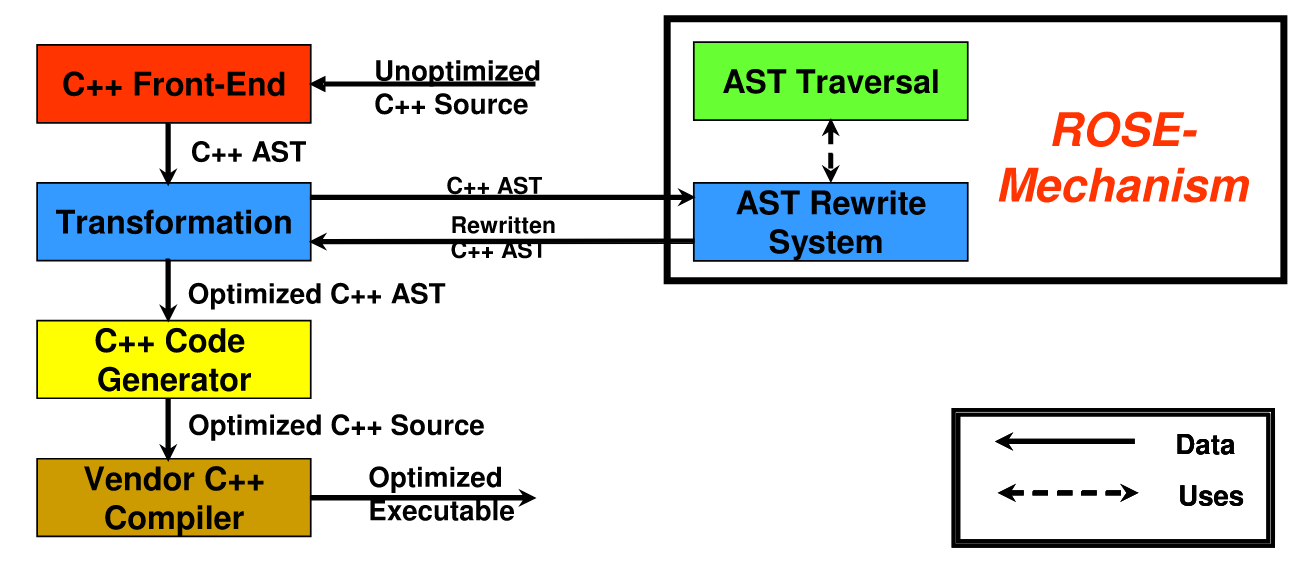
\includegraphics[width=0.7\textwidth]{pictures/rose.png}
    \caption{The ROSE compiler infrastructure.}
    \label{fig:rose}
\end{figure}
The flow diagram in \autoref{fig:rose}  reflects the complete approach, transforming unoptimized C++ code based on user defined abstractions into highly optimized code.
Using the code's Abstract Syntax Tree (AST) representation and leveraging the static analysis capabilities of the ROSE libraries, one can analyze the code and identify opportunities for improvement. This entails identifying particular code style elements, introducing new code segments, modifying or removing existing code, all while preserving the original code's intended semantics.

\begin{figure}[!h]
    \centering
    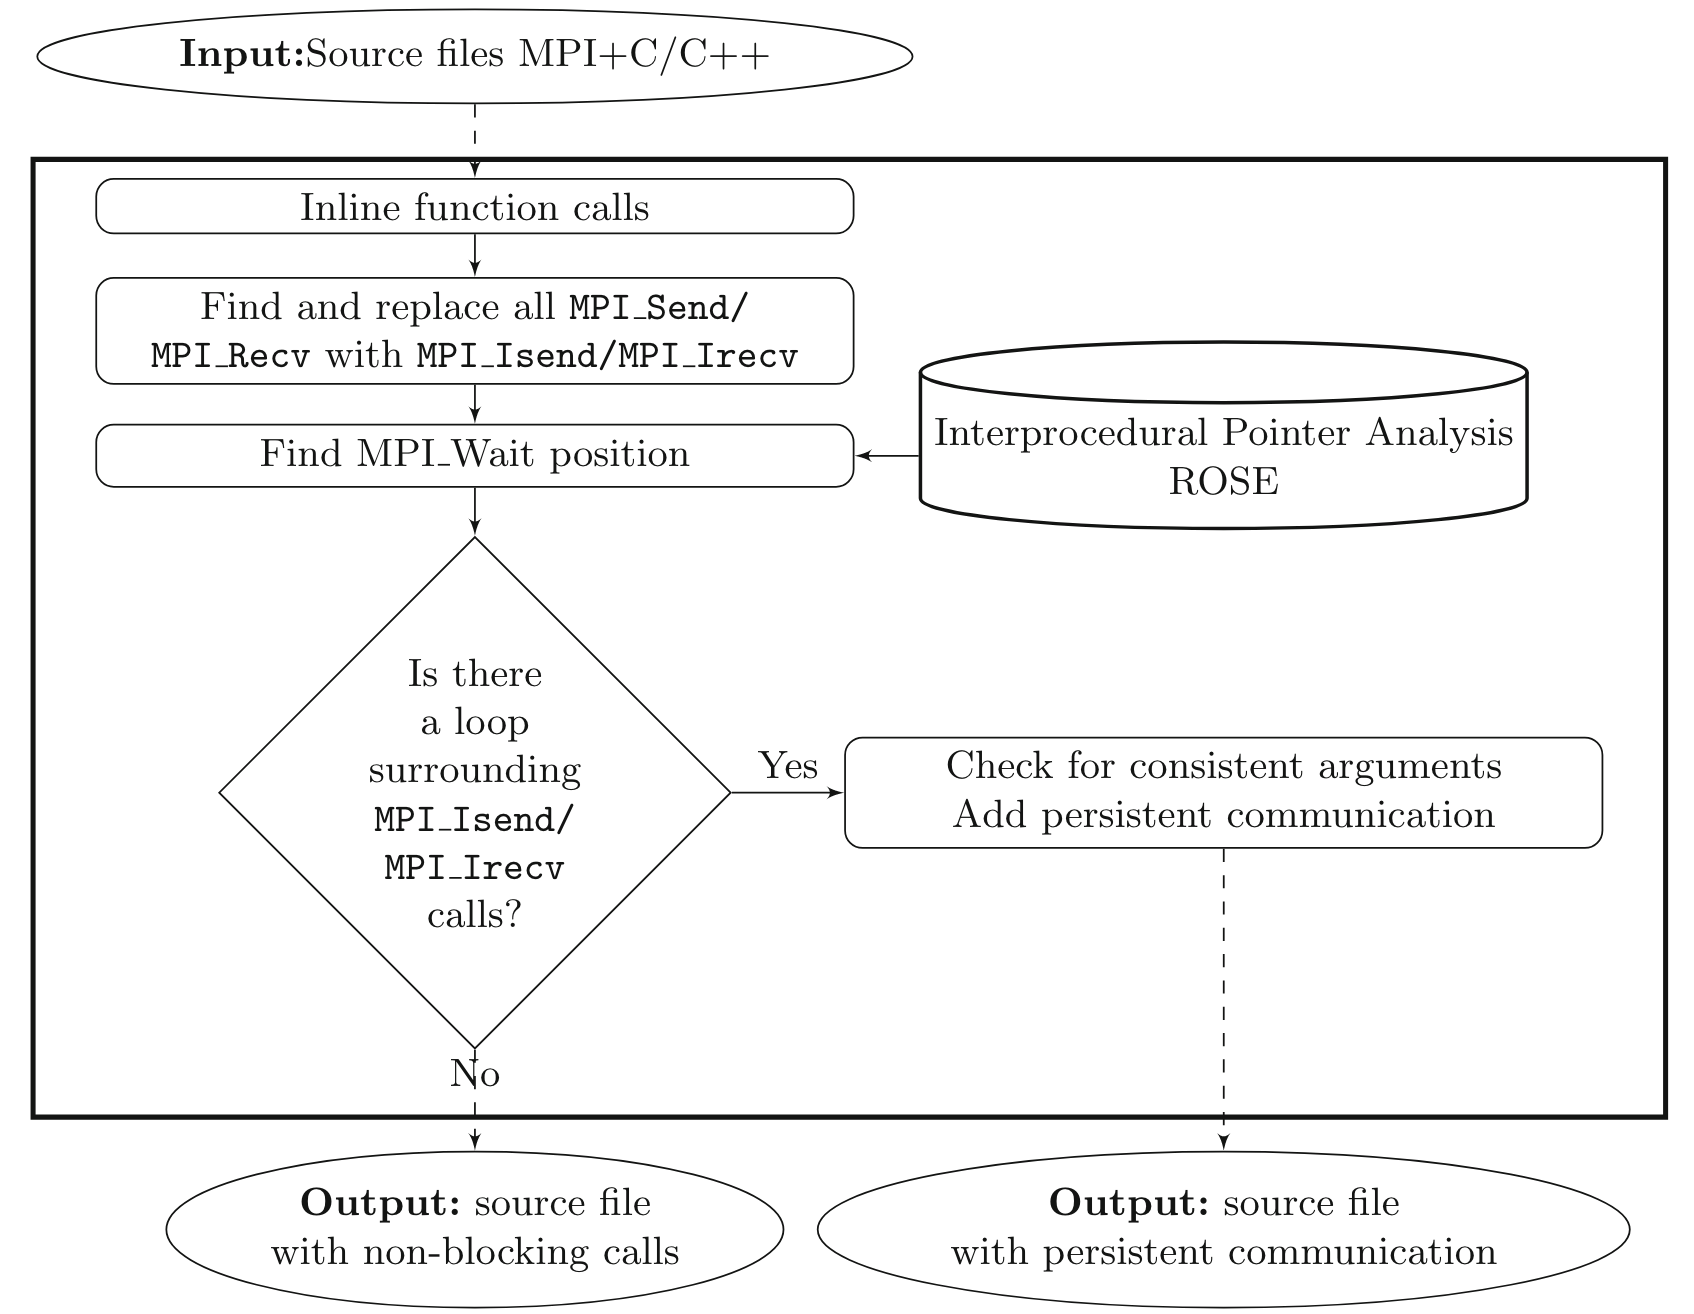
\includegraphics[width=0.7\textwidth]{pictures/petal_p2p_workflow.png}
    \caption{The Petal transformation framework for poin-to-point communications. \cite{ahmed_petal_2016}}
    \label{fig:petal-p2p-workflow}
\end{figure}
An overview of the transformation framework for point-to-point operations is shown in \autoref{fig:petal-p2p-workflow}. 
With transformations for collective operations, after inlining functions, Petal will perform some addition analysis. Transformation framework for colective operations is illustrated in \autoref{fig:petal-collective-workflow}. Petal will count the number of calls to blocking collectives within each block. 
The count is needed to allocate the maximum number of \texttt{MPI\_Request} and status objects that are needed, and reuse the same request for communications on mutually exclusive paths. 
If the function implementation is available, the function calls are then inlined. After being inlined, ROSE's query and builder libraries are used to locate blocking calls, replace them with non-blocking ones, and determine where to put \texttt{MPI\_Wait()} calls in their place. 
These non-blocking calls are replaced with persistent communication operations if any or all of them are invoked again with the same parameters. 
Petal ultimately creates a new source code, utilizing either persistent communications (which are always non-blocking) or non-blocking communications.  Following this strategy is based on the need to increase communication and computation overlap without sacrificing the original application's semantics.
\subsubsection{Blocking to Non-blocking Transformation}
To provide proper access to message buffers, Petal permits the replacement of the blocked function calls \texttt{MPI\_Send} and \texttt{MPI\_Recv} with their corresponding \texttt{MPI\_Isend} and \texttt{MPI\_Irecv}. 
In order to ensure the safety of the data, Petal inserts \texttt{MPI\_Wait} before any operations that access the message buffer. \cite{ahmed_petal_2016}

\subsubsection{Transformation of Point-to-Point Communication}

The basic point-to-point communication operations are send and receive with corresponding blocking function  \texttt{MPI\_Send} and \texttt{MPI\_Recv} in C binding. 
Calling \texttt{MPI\_Send/MPI\_Recv} is in effect the same as calling \texttt{MPI\_Isend/MPI\_Irecv} immediately followed by \texttt{MPI\_Wait()}.

Three variables are constructed to replace each blocking call with its matching non-blocking alternative. 
Two of these variables serve as handlers for \texttt{MPI\_Request} and \texttt{MPI\_Status}. The third variable is a flag added to ensure the \texttt{MPI\_Wait} of the corresponding non-blocking call is correctly executed. 
Instead of each blocking call, \texttt{MPI\_Isend/MPI\_Irecv} are used instead. The next step is to identify the subsequent statements, extract the variables utilized within those statements, and perform pointer analysis to look for any potential aliasing between the variables at hand and the message buffer. 
Petal recognizes probable update activities while dealing with send operations, such as variables that occur on the left-hand side of assignments. 
Petals use the pointer alias analysis from ROSE infrastructure to check the possibilities for an update could modify some data.

Petal shifts the \texttt{MPI\_Wait} operation downwards along the forward control flow edges, ensuring the safety of operations concerning MPI operations and buffer access. 
To ensure code correctness, any write made to a message buffer utilized in a send operation or any access to a message buffer employed in a receive operation is classified as an unsafe access, requiring a prior call to \texttt{MPI\_Wait}.

When dealing with the receive operation, all expressions that retrieve values from variables are tested.
Array subscripts, arguments used in non-inlined function calls, variables used in conditional statements, initial, and increment statements inside for loops, and operands of binary and unary operations are all included in the extraction of variables. 
Petal uses ROSE's pointer alias analysis again to check whether the extracted variables and the communication buffer possibly refer to the same memory location, in order to identify any potential aliasing. 
The tool places the corresponding \texttt{MPI\_Wait} before the statement that makes use of this variable if aliasing is a possibility.

Petal can continue its search for potential uses of the message buffer outside the function that contains the original MPI calls after the function has ended, due to the previously executed inlining.  
If no alias is detected, the \texttt{MPI\_Wait} will consequently be added before the \texttt{MPI\_Finalize} call. 
Due to the complexity of data dependencies carried by loops, the tool does not currently support moving \texttt{MPI\_Wait} outside of a loop's body.

\lstinputlisting[language=C++, caption={Point-to-point blocking version.}, label={lst:p2p_blocking}]{listing/p2p_blocking.cpp}

\autoref{lst:p2p_blocking} shows an example of a code snippet, which uses blocking point-to-point communication and \autoref{lst:p2p_non-blocking} shows the non-blocking version of the code after transformation.
On line 3-5, the tool creates three variables to keep track of the state of the calls. Line 13 shows that the blocking call is replaced with the non-blocking call with corresponding parameters. Before executing the \texttt{MPI\_Wait} on Line 22, 
Line 21 checks to see if the flag is set to 1, which is done in Line 11. The \texttt{printf} function call is a safe read access because this is a send call, and the wait call is added after it.


\lstinputlisting[language=C++, caption={Transformed non-blocking point-to-point version.}, label={lst:p2p_non-blocking}]{listing/p2p_non-blocking.cpp}

\subsubsection{Transformation of Collective Communication}
\phantomsection\label{sssec:collective_communication}
For collective communications, the schema for transformation is similar to for point-to-point, with some additional analysis:

\begin{figure}[!h]
    \centering
    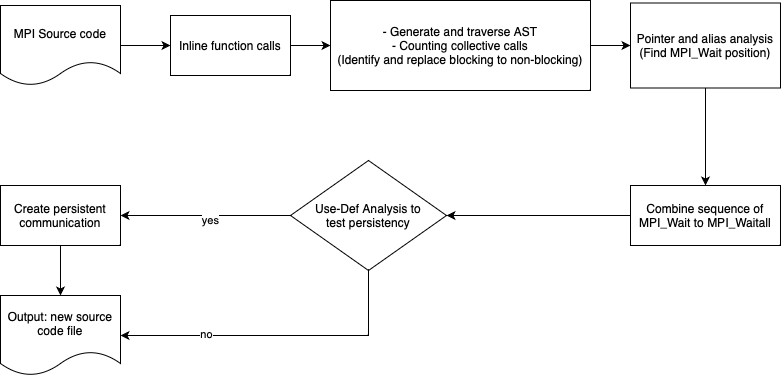
\includegraphics[width=0.7\textwidth]{pictures/petal_collective-workflow.png}
    \caption{The Petal transformation framework for collective communications. Adapted from \cite{ahmed_transforming_2017}}
    \label{fig:petal-collective-workflow}
\end{figure}

After inlining all the function calls, within each block, calls to blocking collectives will be counted. 
The count is required in order to reuse the same request for communications on mutually exclusive paths and allocate the necessary number of \texttt{MPI\_Request} and status objects. 

Rose's built-in CodeThorn \cite{margaria_verification_2014} analysis tool offers methods for creating a data flow analysis (DFA) that counts and keeps track of the locations of MPI blocked functions. 

Once Petal has determined the total number of MPI calls, it allocates the necessary request and status objects in the form of two arrays at the beginning of the main function; one for \texttt{MPI\_Request} which is set to \texttt{MPI\_REQUEST\_NULL}, and the other for \texttt{MPI\_Status}. Finally, Petal transforms the blocking collective calls to non-blocking collective primitives. 

To this end, it changes the blocking function calls to the corresponding non-blocking function. In addition, it appends the \texttt{MPI\_Request} object to the argument list. The request handle is an element from the request array with the index subscript assigned by DFA.

The next step is to locate an area where \texttt{MPI\_Wait} can be inserted that provides sufficient communication-computation overlap. 
The more computation we can overlap with communication, the better we can hide costs associated with communication.
One or two references to message buffers are required as arguments for MPI communication calls. Because of this, Petal makes use of pointer alias analysis to identify code that adds dependencies.  
For each collective call that follows a collective MPI call, Petal collects read and write variables.

If the buffer or its aliases is among the write variables, then the statement is considered unsafe. 
The \texttt{MPI\_Wait} that concludes the collective call has to be inserted before it.

For a read variable, this requirement can be relaxed under certain conditions. If the buffer is used only for sending, a read does not introduce an unsafe dependency and the \texttt{MPI\_Wait} can be moved across it. However, if it is a receive buffer, then the read introduces a true dependency and the \texttt{MPI\_Wait} has to be inserted before it.

\lstinputlisting[language=C++, caption={Positions for \texttt{MPI\_Wait}}, label={lst:rank_blocking}]{listing/rank_blocking.cpp}

\break

Petal considers the fact that most collective operations involve two buffers in communication. 
In certain operations like \texttt{MPI\_Reduce} and \texttt{MPI\_Scatter}, one of the buffers only plays a role at the root process and is not involved in communication with other processes. 
In \texttt{MPI\_Reduce}, the receive buffer is significant only for the root rank, whereas in \texttt{MPI\_Scatter}, it is the send buffer. 
The reason why the \texttt{MPI\_Wait} call can be different for root and non-root processes root MPI is due to the difference in communication patterns and responsibilities between these two types of processes.
Root processes may need to wait for multiple communication operations to complete before proceeding. For example, if the root process is collecting data from non-root processes, it may need to wait for all the non-root processes to send their data before it can proceed with the data collection. 
Meanwhile, non-root processes typically perform a specific computation or send their results to the root process or processes usually have a simpler communication pattern, often involving a single ``send'' or ``receive'' operation.
Non-root processes usually have a simpler communication pattern, often involving a single ``send'' or ``receive'' operation.
\autoref{lst:rank_blocking} illustrates an example where the optimal placement of \texttt{MPI\_Wait} depends on whether the process is the root or not. 
Petal calculates the appropriate position for \texttt{MPI\_Wait} for both the root rank and other ranks. 
If the computed positions are the same, Petal simply uses \texttt{MPI\_Wait}. However, if the positions differ, it inserts \texttt{MPI\_Wait} at both positions, protected by a condition that checks the rank against the MPI process. 
This allows non-root ranks to proceed with computation in certain cases, while the root rank must wait for the completion of scatter or reduce, as depicted in \autoref{lst:rank_non-blocking}.

\lstinputlisting[language=C++, caption={Transformed non-blocking code}, label={lst:rank_non-blocking}]{listing/rank_non-blocking.cpp}

In case, if a function call cannot be inlined, due to it its implementation not being available, Petal analyzes the call's arguments. 
If one of them relates to the message buffer in question, Petal treats this call as unsafe. 
Otherwise, the call is considered independent and can be overlapped safely with communication. 
The exception to this rule are calls to other MPI functions. Since MPI is a standard specification, Petal understands its API and arguments. 
Petal has stored information for each MPI function in arrays and whether an argument is read or written. 
Using this information as part of the message buffer analysis, Petal decides whether concurrent communications are feasible or not. 
If there is no dependency between all the communication message buffers, (i.e., only sending buffers can be identical), communication calls can overlap as well. 

\lstinputlisting[language=C++, caption={Blocking concurrent communication.}, label={lst:blocking_collective_cc}]{listing/collective_cc_blocking.cpp}

\autoref{lst:blocking_collective_cc} shows an example of this case. 
By looking at the message buffer of the three consecutive \texttt{MPI\_Bcast} for \texttt{foo}, \texttt{bar}, \texttt{foobar}, Petal is able to detect that they are all distinct and hence can be safely overlapped. 
\autoref{lst:non-blocking_collective_cc} shows the transformation's output.

\lstinputlisting[language=C++, caption={Transformed non-blocking concurrent communication.}, label={lst:non-blocking_collective_cc}]{listing/collective_cc_non-blocking.cpp}

Petal considers certain operations, such as \texttt{MPI\_Wtime}, \texttt{MP\_Barrier}, and \texttt{MPI\_Finalize}, to be special operations that cannot be overlapped with communication. 
Therefore, any communication that starts before calling these functions must be completed before executing these special operations. 
Petal includes \texttt{MP\_Wait} just before any of these special operations. 
To ensure that the \texttt{MPI\_Wait} is executed only when its corresponding nonblocking call is executed, Petal checks if the nonblocking initiation and wait for completion occur within the same scope. 
If they are in different scopes, Petal utilizes a flag that is set to true after initiating a nonblocking call. 
The corresponding \texttt{MPI\_Wait} is protected by a condition that checks if the flag is true. 
Once the wait operation is executed, the flag is reset. This ensures that the wait operation is executed only if the initiation call has been executed.

After locating every position for \texttt{MPI\_Wait}, Petal checks to see whether they can all be combined into one position. 
If there are no other active communications, Petal replaces each individual call that uses a series of request objects in a multiple wait call with a single 
\texttt{MPI\_Waitall} call. By comparing the subscript values of the requests in the set with the wait positions, Petal makes sure the requests are consecutive. 
Petal determines if there is at least one current communication with a different wait position and decides to insert each wait call separately if the difference between the maximum and minimum subscript values plus one does not equal the number of identified wait calls.

\autoref{collective_blocking} shows the code for solving $A \cdot x = b$ using the conjugate gradient method [source]. \autoref{collective_non-blocking} then illustrates how Petal transformed this code to its non-blocking version.
After inlining and counting collective calls, Petal creates corresponding arrays \texttt{reqs[2], flags[2]} and \texttt{stats[2]} in order to keep track of states for the calls. 

Petal detected that the arguments of \texttt{MPI\_Allgather} in line 14 are independent from the arguments of \texttt{SolvePrecondMatrix}, \texttt{ComputeVectorDotProduct} and the array \texttt{Bloc\_Delta1}. As a result, its \texttt{MPI\_Wait} with corresponding buffer can be placed at the end of the loop.
This collective call is also separate from collecting \texttt{Delta1} as well.
So that, its \texttt{MPI\_Wait} with corresponding buffers can be placed at the end of the loop.

No other independent processing is identified because an argument to the \texttt{MPI\_Iallreduce} message is used immediately after the call. 
The receive buffer in this call is represented by \texttt{\&Delta1}. 
Since Line 18's computation reads from \texttt{Delta1}, it cannot begin before \texttt{Delta1} has been computed.

\lstinputlisting[language=C++, caption={Example with collective blocking communications}, label={collective_blocking}]{listing/collective_blocking.cpp}

\lstinputlisting[language=C++, caption={Transformed non-blocking collective version}, label={collective_non-blocking}]{listing/collective_non-blocking.cpp}

